\documentclass[border=4pt]{standalone}
\usepackage{tikz}
\usetikzlibrary{shapes.geometric}
\begin{document}
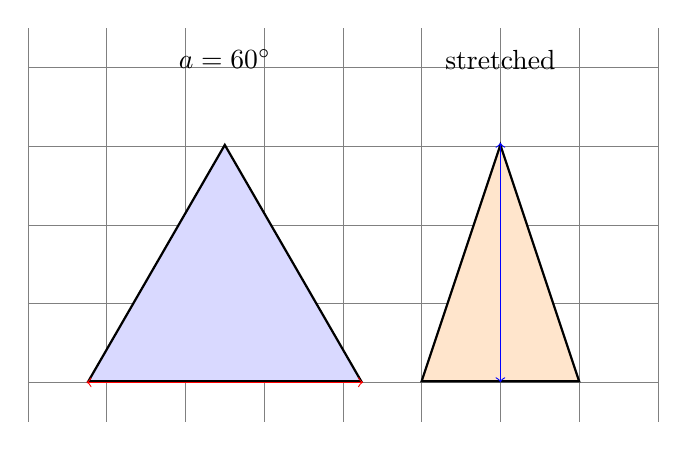
\begin{tikzpicture}[
  tri/.style={
    isosceles triangle,
    isosceles triangle apex angle=60,
    inner sep=0pt,
    draw,
    thick,
    anchor=lower side,
    shape border rotate=90
  }
]
  \draw[help lines] (-1,-0.5) grid (7,4.5);
  \node[tri,minimum height=3cm,fill=blue!15] (fixed) at (1.5,0) {};
  \node[tri,isosceles triangle stretches,minimum width=2cm,minimum height=3cm,fill=orange!20] (stretched) at (5,0) {};
  \draw[red,<->] (fixed.left corner) -- (fixed.right corner);
  \draw[blue,<->] (stretched.lower side) -- (stretched.apex);
  \node at (1.5,4.1) {$a=60^\circ$};
  \node at (5,4.1) {stretched};
\end{tikzpicture}
\end{document}
